\begin{frame}{GRUs}
\centering
        \begin{tikzpicture}
            \tikzset{layer/.style={draw,rectangle, fill=gray!20, thick}}
            \tikzset{edge/.style={->, thick}}
        
            \node(x1) at (0,0) [layer, minimum width=2cm] {$\bm{x_1}$};
            \node(h1) at (0,2) [layer, minimum width=1.5cm] {$\bm{h_1}=\texttt{GRU}(.)$};
            \node(y1_hat) at (0,4) [layer, minimum width=1cm] {$\bm{\hat{y_1}}$};
            \draw[edge](x1) -- node[left]{$\bm{U}$} (h1);
            \draw[edge](h1) -- node[left]{$\bm{V}$} (y1_hat);
        

            \node(x2) at (3,0) [layer, minimum width=2cm] {$\bm{x_2}$};
            \node(h2) at (3,2) [layer, minimum width=1.5cm] {$\bm{h_2}=\texttt{GRU}(.)$};
            \node(y2_hat) at (3,4) [layer, minimum width=1cm] {$\bm{\hat{y_2}}$};
            \draw[edge](x2) -- node[left]{$\bm{U}$} (h2);
            \draw[edge](h2) -- node[left]{$\bm{V}$} (y2_hat);
        
            \node(x3) at (6,0) [layer, minimum width=2cm] {$\bm{x_3}$};
            \node(h3) at (6,2) [layer, minimum width=1.5cm] {$\bm{h_3}=\texttt{GRU}(.)$};
            \node(y3_hat) at (6,4) [layer, minimum width=1cm] {$\bm{\hat{y_3}}$};
            \draw[edge](x3) -- node[left]{$\bm{U}$} (h3);
            \draw[edge](h3) -- node[left]{$\bm{V}$} (y3_hat);
        
            \node(etc) at (8,2) [] {...};
            
            \draw[edge, myblue] (h1) --  (h2);
            \draw[edge,myblue] (h2) --  (h3);
            \draw[edge,myblue] (h3) -- (etc);
        
        \end{tikzpicture}
\end{frame}
\begin{frame}{GRU}
    \centering
    \begin{figure}
        \centering
        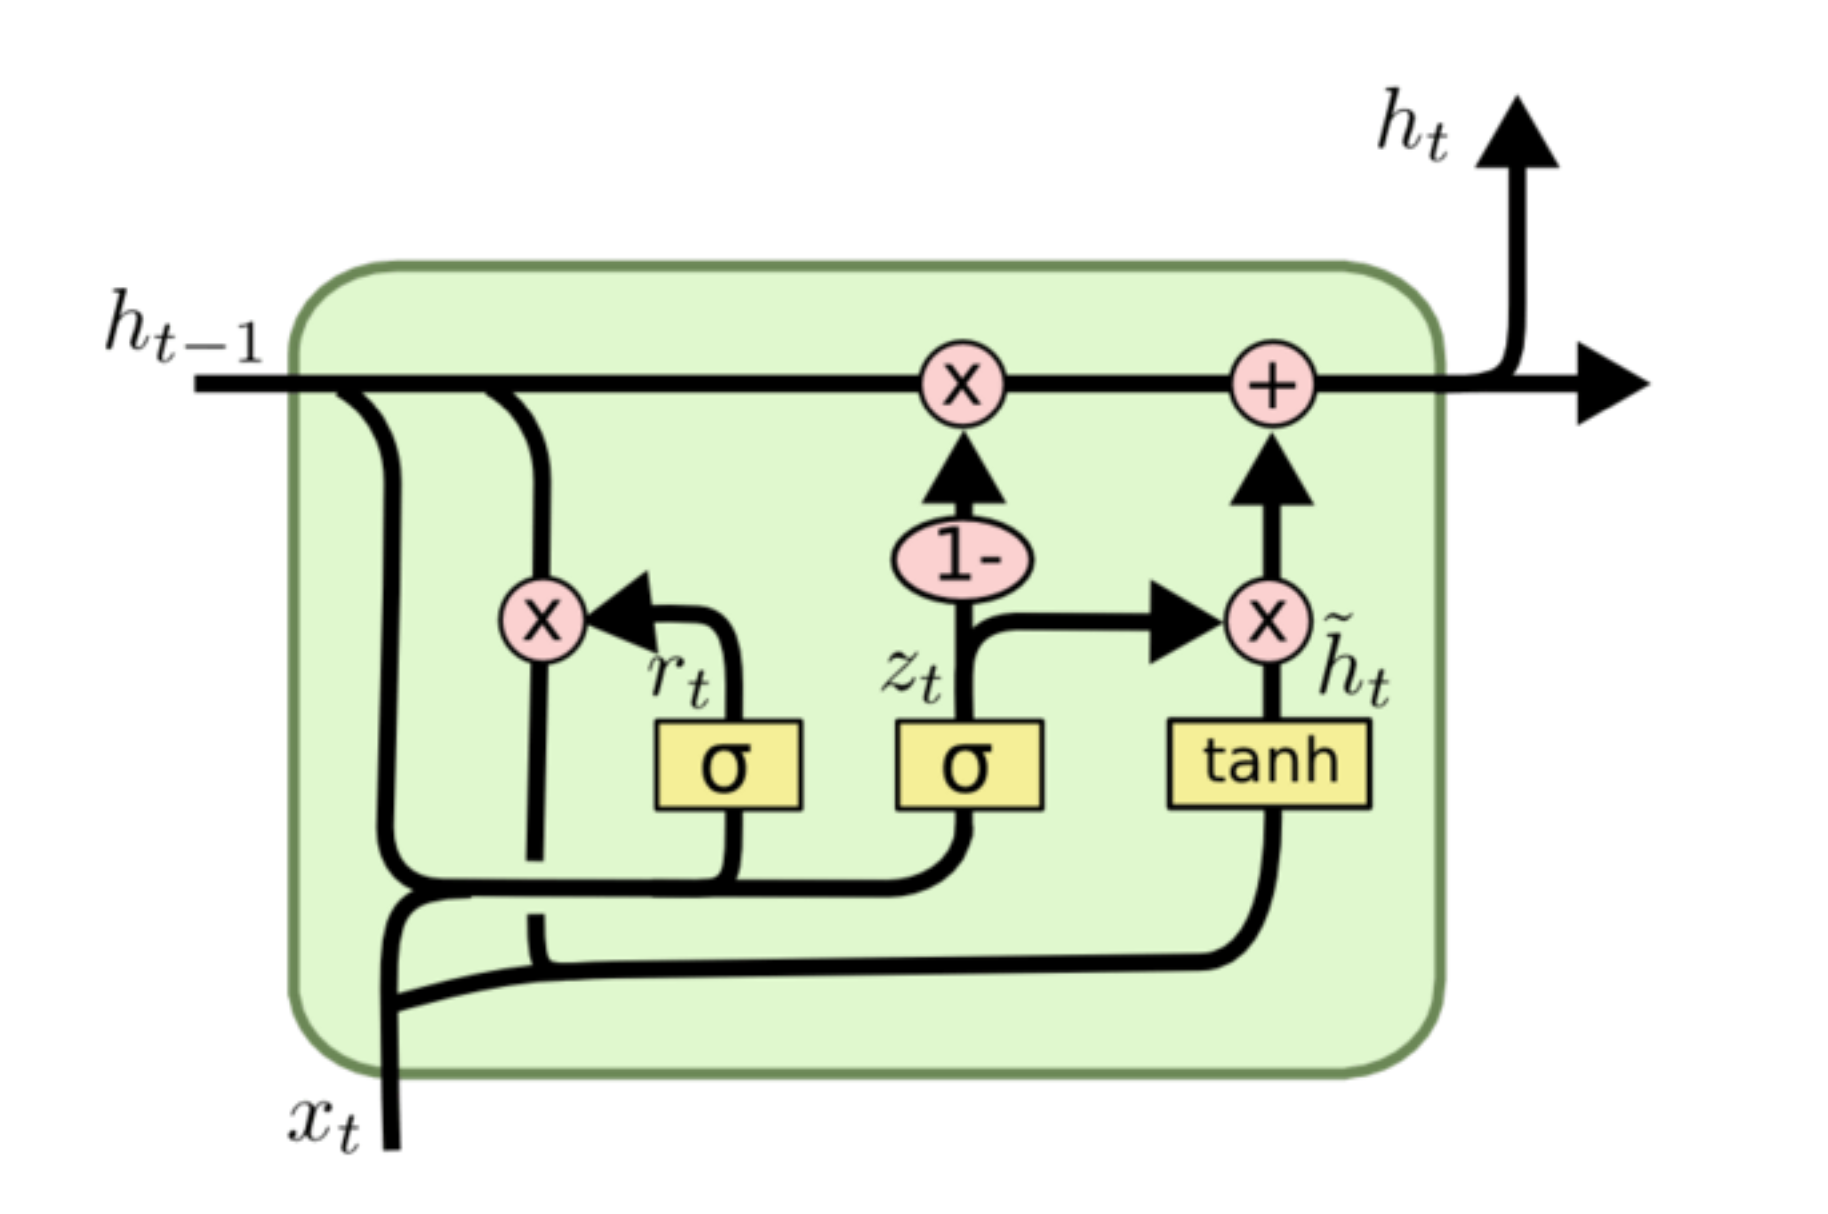
\includegraphics[scale=0.2]{./figure/gru.png}
    \end{figure}
    \begin{itemize}
        \item reset gate $r_t = \sigma ( \bm{x_t} \bm{U^{(r)}} + \bm{h_{t-1}} \bm{W^{(r)}} )$
        \item new memory content could be $\bm{\tilde{h}_t} = \texttt{tanh} ( \bm{x_t} \bm{U} + \bm{h_{t-1}} \bm{W} 
        \odot r_t)$ 
        \item update gate $z_t = \sigma ( \bm{x_t} \bm{U^{(z)}} + \bm{h_{t-1}} \bm{W^{(z)}} )$
        \item final memory encodes a combination of current content and its content in the previous time step
         $\bm{h_t} = (1-z_t) \odot \bm{h_{t-1}} + z_t \odot \bm{\tilde{h}_t}$
    \end{itemize}
\end{frame}
\begin{frame}{GRU: Extreme Cases}
    \centering
    \begin{itemize}
        \item reset gate $r_t \in {0,1}$
        \item update gate $z_t \in {0,1}$
        \item If $z_t = 0$
        \begin{itemize}
            \item $\bm{h_t} = (1-z_t) \odot \bm{h_{t-1}} + z_t \odot \bm{\tilde{h}_t}$ 
            \item $\bm{h_t} = \bm{h_{t-1}}$
            \item zero gradients over different time steps 
            \item no vanishing gradients
        \end{itemize}
        \item If $z_t =1$
        \begin{itemize}
            \item $\bm{h_t} = (1-z_t) \odot \bm{h_{t-1}} + z_t \odot \bm{\tilde{h}_t}$ 
            \item $\bm{h_t} = \bm{\tilde{h}_t}$
            \item  $\bm{\tilde{h}_t} = \texttt{tanh} ( \bm{x_t} \bm{U} + \bm{h_{t-1}} \bm{W} \odot r_t)$ 
            \item If $r_t=0$
            \begin{itemize}
                \item $\bm{h_t} = \texttt{tanh}(\bm{x_tU})$ 
                \item forget past
            \end{itemize}
            \item If $r_t =1$
                \begin{itemize}
                    \item $\bm{h_t} = \texttt{tanh} ( \bm{x_t} \bm{U} + \bm{h_{t-1}} \bm{W}) $
                    \item a standard RNN gate
                \end{itemize}
        \end{itemize}
    \end{itemize}
\end{frame}

\begin{frame}{Long Short-Term Memory (LSTMs)}
\begin{itemize}
    \item LSTMs were introduced by Hochreiter and Schmidhuber (1997)
    \item LSTMs contains more parameters than what GRU has
\end{itemize}
\end{frame}

\begin{frame}{LSTM Unit}
\centering
    \begin{figure}
        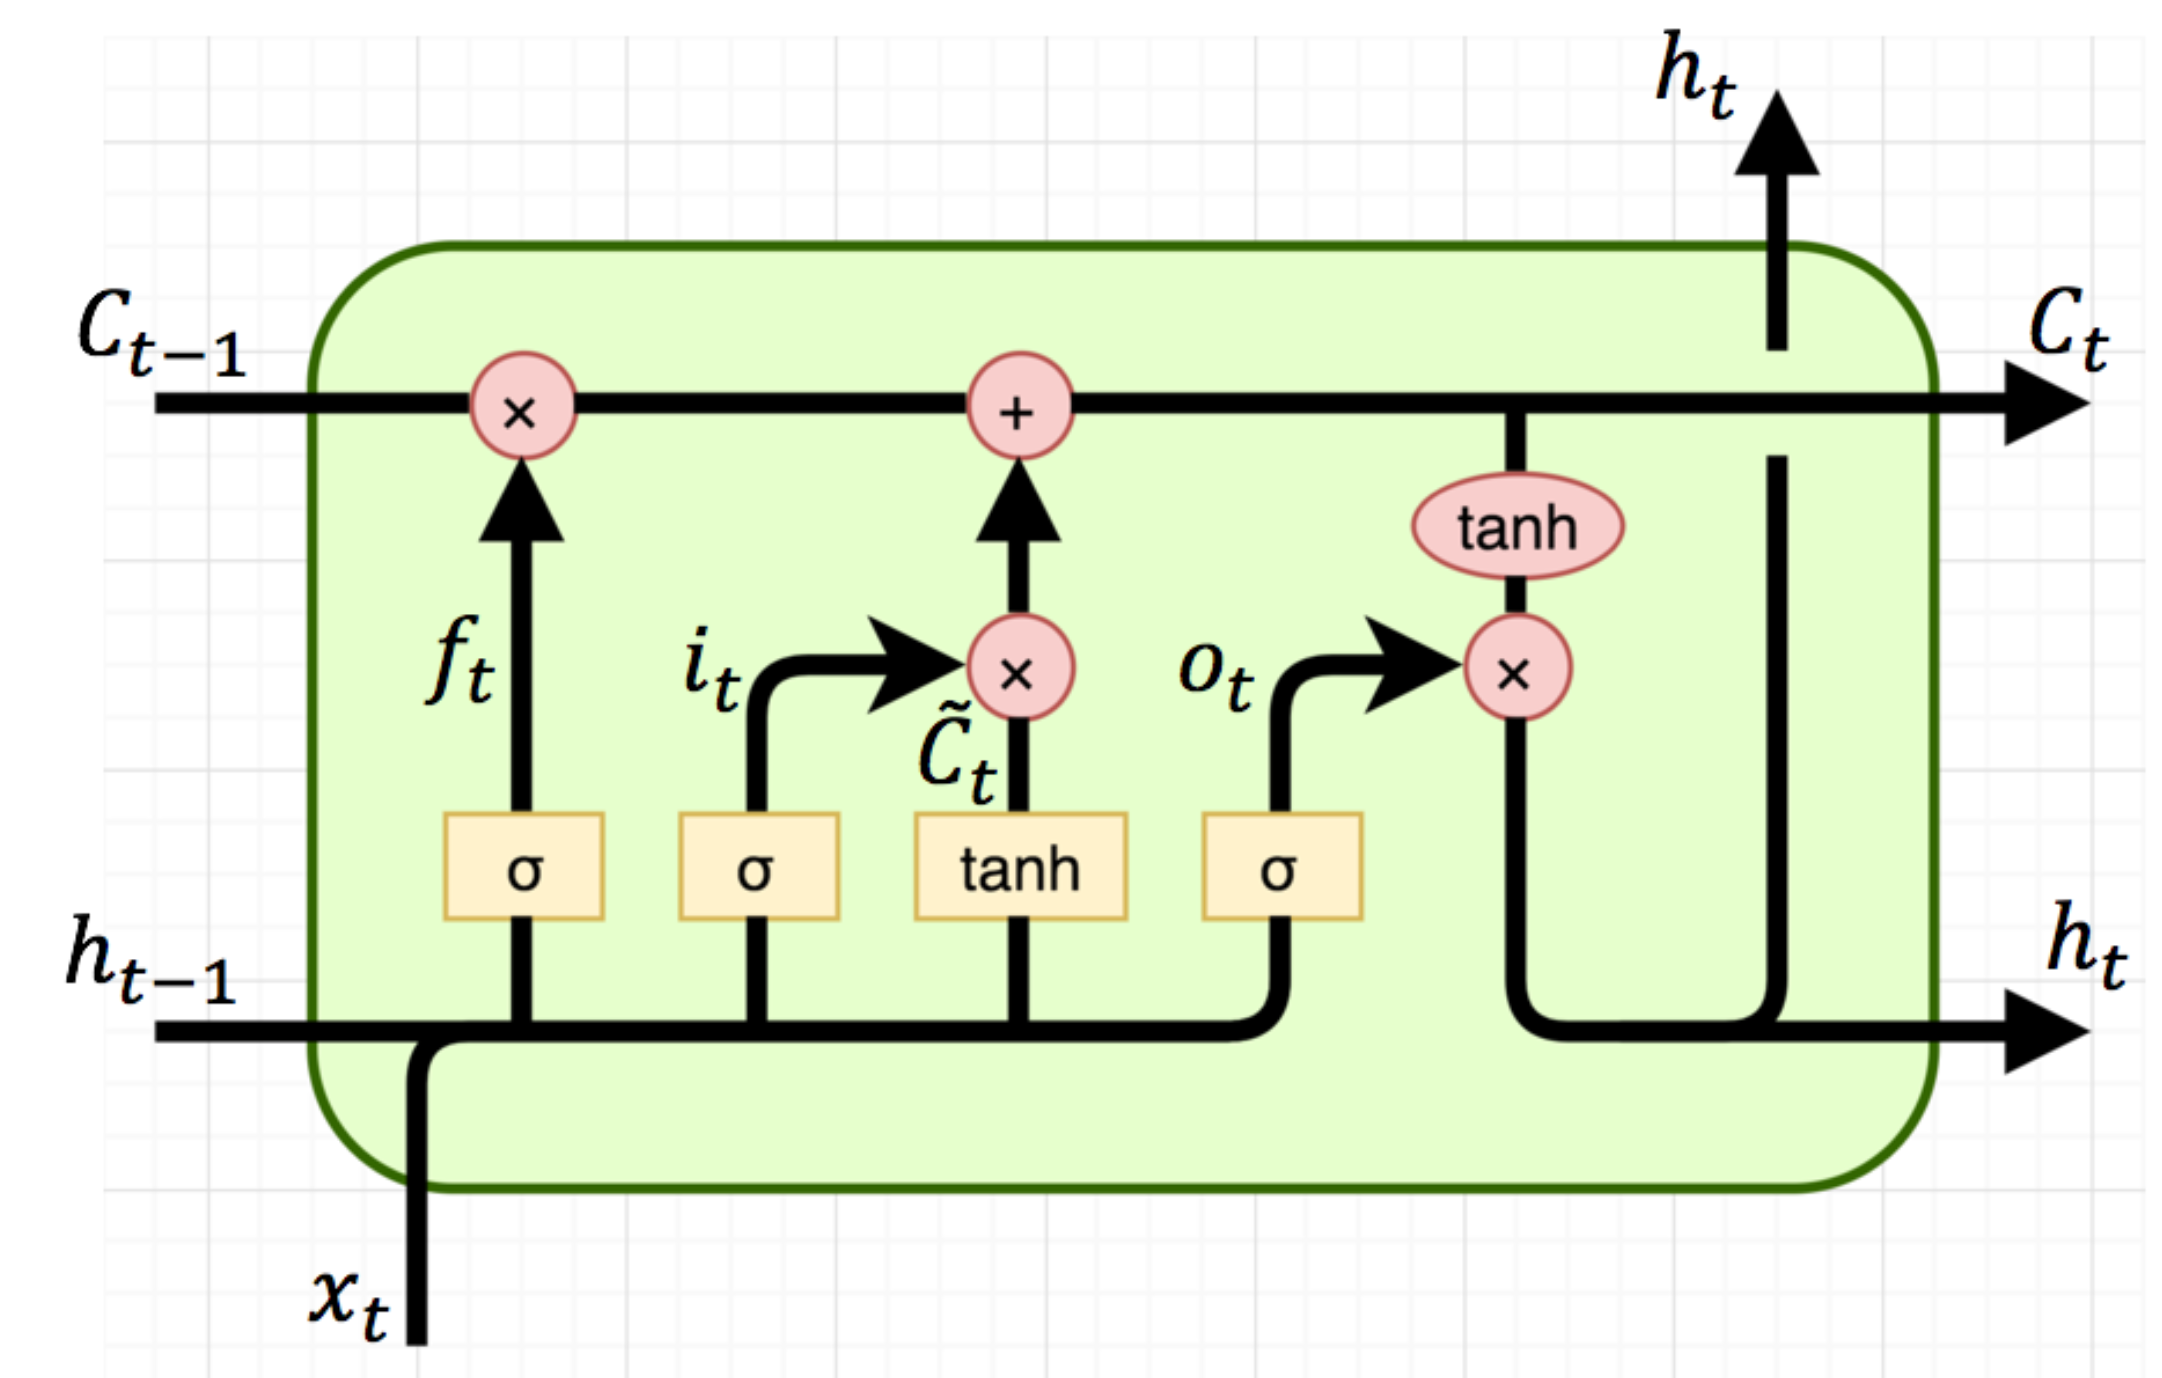
\includegraphics[scale=0.15]{./figure/lstm.png}
    \end{figure}
    \begin{itemize}
        \item Input gate (=write gate) $i_t = \sigma \big( \bm{x_tU^{(i)}} + \bm{h_{t-1}W^{(i)}}   \big) $
        \item Forget gate (=reset gate) $f_t = \sigma \big( \bm{x_tU^{(f)}} + \bm{h_{t-1}W^{(f)}}   \big) $
        \item Output gate (=read gate) $o_t = \sigma \big( \bm{x_tU^{(o)}} + \bm{h_{t-1}W^{(o)}}   \big) $
        
        \item New memory cell is $\bm{\tilde{c}_t} = \texttt{tanh} ( \bm{x_tU}+\bm{h_{t-1}W} ) $
        \item Final memory cell is $\bm{c_t} = f_t \odot \bm{c_{t-1}} + i_t \odot \bm{\tilde{c}_t}$
        \item Final hidden state is $\bm{h_t} = o_t \odot \texttt{tanh}(c_t)$
    \end{itemize}
\end{frame}
